\documentclass{book}
\usepackage[paperwidth=148mm,paperheight=110mm,text={148mm,160mm},left=0mm,top=10pt]{geometry}
\usepackage{ctexcap}
\usepackage[labelfont=bf,labelsep=quad]{caption}
  \DeclareCaptionFont{kai}{\kaishu}
  \captionsetup{textfont=kai}
\usepackage{graphicx,floatrow,subfig}
\renewcommand{\rmdefault}{ptm}
\begin{document}
\setcounter{chapter}{2}
\songti

\begin{figure}[!h]
\centering
\subfloat[��·ͼ]{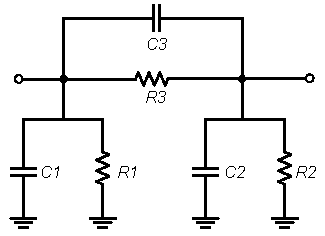
\includegraphics{fig44.pdf}}\hspace{30pt}
\subfloat[Ԫ����]{\begin{tabular}[b]{cccc}\hline
C1  & 0.36pF & R1 & 1.5k \\
C2  & 0.22pF & R2 & 8.2k \\
C3  & 0.11pF & R3 & 4.7k \\ \hline\vspace{3mm}
\end{tabular}}\\
\subfloat[Ƶ������]{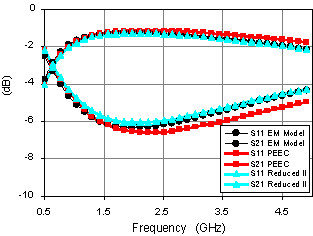
\includegraphics{fig46.pdf}}\hspace{30pt}
\subfloat[Q ֵ����]{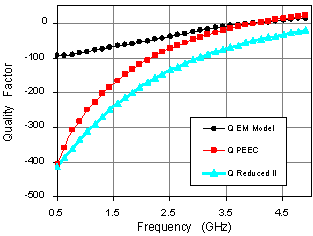
\includegraphics{fig45.pdf}}
\caption{$\pi$ ��~RC ��������·}
\end{figure}
\end{document}
